\chapter{Experiments\label{chap:exp}}

The overhead introduced by oxc framework includes three parts:
\begin{itemize}
\item The time required to execute codes brought oxc functions.
\item The context switches introduced by the oxc framework.
\item The degradation of modular schedulers' performance under oxc 
	framework.
\end{itemize}

The third item is caused by implementation limitation can be minimized 
or removed by improving implementation details. For example, to access 
the per CPU runqueue in Linux is an optimized operation. However, the 
access to a per ox container is not so efficient, this will give a 
penalty when scheduler works inside an ox container.

There are two experiments carried out to evaluate the overhead in the 
oxc framework. In experiment A, the code execution time of frequently 
invoked oxc functions is measured. In experiment B, the overall overhead 
of oxc control is estimated through comparisons with rt throttling and 
cfs bandwidth control.

Inside each oxc function, there is a scheduling operation inside and
codes to regulate bandwidth reservation. The cost of these functions 
is the main interest in experiment A. Current oxc framework 
implementation is still a prototype. Some kernel features are not 
considered under the framework yet. For instance, the 
\texttt{priority inheritance}, which is important for the kernel's 
real-time performance and will influence number of context switches. 
So, instead of counting and analyzing context switches directly,
in experiment B the overhead of scheduling inside an ox container is
approximately evaluated by a relative way. As for the context switches 
caused by importng CBS based scheduling in the kernel, people can refer  
to \cite{Luigi09} for more iformation; yet these results do not straightly 
apply to oxc work. 

The hardware and software used in the experiment are shown in 
table \ref{tab:exp_setup}.
\begin{table}[H]%thbp]
  \centering
  \begin{tabular}{ll}\hline
	\emph{Hardware platform}\hspace{4cm}		& 	\\
	Processor			& Intel(R) Core(TM) Duo E8500	 \\
	Frequency			& 3.16GHz\\
	RAM				& 	  \\	
					&	\\	
	\emph{Software platform}\hspace{4cm}		& 	\\
	Linux distribution		& Ubuntu 11.10\\
	Compiler version		& gcc 4.6.1\\
	Kernel version			& 3.4.0-rc+ \\\hline
  \end{tabular}
  \caption{Hardware-Software platform}
  \label{tab:exp_setup}
\end{table}
The chapter is organized like this: the tracing tool and synthetic 
benchmark tool we use in the experiment are described; then it's the 
design and result analysis of each experiment; finally, what we learn
from the experiment is concluded.

\section{Ftrace in Linux kernel}
Ftrace\cite{ftrace} is an internal tracer designed to help out developers of systems to
find out what is going on inside the kernel. The name ftrace comes from
''function tracer'', which is its original purpose and the reason it is 
used here. Now there are various kinds of tracers incorporated in Ftrace.
You can use it to trace context switces, hong long interrupts are disabled,
and so on.

Ftrace uses \emph{debugfs} file system to hold control files as well as
file to display output. 
Typically, ftrace is mounted at \texttt{/sys/kernel/debug}.
\begin{lstlisting}
	#mount -t debugfs nodev /sys/kernel/debug
\end{lstlisting}
After this command, a directory \texttt{/sys/kernel/debug/tracing} will 
be created containing interfaces to configure ftrace and display results.
\begin{lstlisting}
	#cd /sys/kernel/debug/tracing
\end{lstlisting}
The following commands will be assumed to be called under \texttt{tracing}
directory.
There are several kinds of tracers available in ftrace, simply cat the
\texttt{available\_tracers} file in the \texttt{tracing} dorectory.
The output could vary with enabling or disabling kernel configuration 
options concerned with ftrace functionality in compilation time.
\begin{lstlisting}
	#cat available_tracers
	blk function_graph mmiotrace wakeup_rt wakeup function sched_switch nop
\end{lstlisting}
The \texttt{function} is the function tracer. It uses the \texttt{-pg} option
of \texttt{gcc} to have every function in the kernel call a special function
\texttt{mcount()} for tracing all kernel functions. 
The \texttt{function\_graph} is similar to the function tracer except that
the function tracer probes functions on their entry whereas the function 
graph tracer traces on both entry and exit of a function. It is called 
function graph tracer because it provides the ability to draw a graph 
of function calls similar to C code as tracing results. 
This \texttt{function\_graph} is what we use in experiments. 
To enable the function graph tracer, just echo \texttt{function\_graph} 
into the \texttt{current\_tracer} file.
\begin{lstlisting}
	#echo function_graph > current_tracer
\end{lstlisting}
A trace can be started and stopped through configuring \texttt{tracing\_on}
file. Echo 0 into this file to disable the tracer or 1 to enable it. Cat the
file will display whether the tracer is enabled or not.

The output of the trace in held in file \texttt{trace} in a human readable
format. The ftrace will by default trace all functions in the kernel. In
most cases, people only care about particular functions. To dynamically
configure which function to trace, the \texttt{CONFIG\_DYNAMIC\_FTRACE}
kernel option should be set in compilation time  to enable dynamic ftrace. 
Actually, \texttt{CONFIG\_DYNAMIC\_FTRACE} is highly recommanded and defaultly
set because of its performance enhancement. To filter which function to trace
or not, two files are used: \texttt{set\_ftrace\_filter} for enabling the
tracing of a specific function and \texttt{set\_ftrace\_notrace} to 
disable the tracing of some function. A list of available functions that you 
can add to these files is listed in \texttt{available\_filter\_functions}.
In the later experiment, the oxc function \texttt{task\_tick\_oxc} is traced
by setting up like this:
\begin{lstlisting}
	#echo task_tick_oxc > set_ftrace_filter
\end{lstlisting}


\section{Tbench}
The tbench \cite{tbench} benchmark is a tool that measures disk throughput 
for simulated netbench runs. Tbench reads a load description file called 
client.txt that was derived from a network sniffer dump of a real netbench 
run and %produces the filesystem load according to the description file. 
it produces only the TCP and process load and no filesystem calls.
One exmple to run tbench test:
\begin{lstlisting}
	$tbench_srv
	$tbench 2 -t 100
\end{lstlisting}
The \texttt{tbench\_srv} should be invoked before running \texttt{tbench}.
The second command starts two tbench connections with one client thread 
and one server thread in each connection. The two connections will run 
simultaneously and the runtime of the benchmark will be 100 seconds.

\section{Experiment A}
\subsection{The experiment design}
In this experiment, the execution time of oxc functions are measured.
In a Linux system, even if the oxc patch is applied in the kernel, 
when there is no oxc tasks, the system performs as a plain Linux system. 
In such a case, the possible oxc overheads include the code execution time 
in function \texttt{is\_oxc\_task} and the oxc related initialization when 
a scheduling group is created; both are negligible.

During the experiment, the execution time of following oxc functions are 
measured using Ftrace:
\begin{itemize} 
\item \texttt{check\_preempt\_curr\_oxc}
\item \texttt{pick\_next\_task\_oxc}
\item \texttt{put\_prev\_task\_oxc}
\item \texttt{task\_tick\_oxc}
\end{itemize} 
They are most often called oxc functions as they enclose in most frequently
invoked scheduling operations. 
The oxc functions like 
\texttt{enqueue\_task\_rq\_oxc} and \texttt{dequeue\_task\_rq\_oxc} only 
happen when a task enters or leaves an ox container. And are not often
happens in the following experiment set up.
%Inside an
%ox container, enqueue and dequeue of a task still frequently happen.
%However, the performance of scheduling operations of a modular
%scheduler under oxc framework is not an emphasis in this experiment.

There will be six individual tests differing in the number of hyper ox 
containers in the system. In the first test, there is only one hyper 
ox container; then, in each test one more hyper ox container would be 
added. All hyper ox containers in the experiment are identical.
Each hyper ox-container has two ox containers with the same CPU 
reservation parameter $0.1ms/1ms$. Each ox container has one dummy task 
within it. The dummy task simply runs a forever while loop and it is a 
rt task with policy \texttt{SCHED\_FIFO}. This while loop task will 
exhuaust the reservation in its ox container. The scheduling policy is 
arbitrarily chosen without special thoughts. On the contrary, the 
situation for modular scheduling inside an ox container is intentionally
arranged as simple as possible to clarify the effect of oxc framework.

The measured execution time of above oxc functions comprises the time 
consumed by codes involving with the oxc control and operations defined 
in modular scheduler which are encapsulated inside the these functions.
%Here the situation for rt scheduling inside an ox container is very simple.
%And the experiment analysis can focus on oxc control overhead.

\subsection{Experiment results}
The results of six tests are listed in table \ref{tab:exp_res}.
The index of a test indicates the number of hyper ox containers in that 
test. The two fields in the pair are average vaule and standard deviation 
of the measured function execution time in micro seconds.
\begin{table}[thbp]
	\centering
	\begin{tabular}{|l||c|c|c|c|c|c|}\hline
		& \tiny{test1} & \tiny{test2} & \tiny{test3} & \tiny{test4} & \tiny{test5} & \tiny{test6}\\\hline
	\tiny{pick\_next\_task\_oxc} &\tiny{(0.168, 0.083)} &\tiny{(0.155, 0.070)} &\tiny{(0.206, 0.178)} 
							&\tiny{(0.230, 0.215)} &\tiny{(0.211, 0.216)} & \tiny{(0.246, 0.251)} \\\hline
	\tiny{put\_prev\_task\_oxc} &\tiny{(0.827, 0.049)} & \tiny{(0.834, 0.096)}&\tiny{(0.820, 0.103)} &\tiny{(0.801, 0.111)} &
					\tiny{(0.829, 0.146)} & \tiny{(0.852, 0.251)}\\\hline
	\tiny{task\_tick\_oxc} &\tiny{(0.272, 0.192)} & \tiny{(0.275, 0.182)}&\tiny{(0.263, 0.155)} & \tiny{(0.261,0.15)}& \tiny{(0.245,0.158)}& 
					\tiny{(0.249,0.146)}\\\hline
	\tiny{check\_preempt\_curr\_oxc} & - & - & - & - & - & - \\\hline
	\end{tabular}
	\caption{Measured execution time, in micro seconds, of oxc functions\\
				 \indent\hspace{4cm}in the format of \emph{(mean, standard deviation)}}
	\label{tab:exp_res}
\end{table}

The first surprise is from the row for \texttt{check\_preempt\_curr\_oxc}. 
That is, no tracing result for \texttt{check\_preempt\_curr\_oxc} is 
recorded. An analysis of overhead in this function is necessary.
The details of this function is in list \ref{check_preempt}.
There are three cases when to check if a task can preempt the currently 
running task. When only one of the two is an oxc task or both two are oxc 
tasks and not in the same ox containers, the comparison cost is just several 
\texttt{if-else} instructions. If they are two oxc tasks in the same container, 
this function follows the procedure in Linux scheduling; in addition, in our 
experiment setup, there is only one task inside an ox container. In short words, 
this function is not a significant soure for oxc framework overhead in tests. 
Although this could be a reason to explain that the ftrace fails to measure
the execution time of \texttt{check\_preempt\_cur\_oxc} during tests, it reminds
us that, given the feature of hierarchical scheduling, it may be attractive to
develop a new recording tool so as to evaluate the oxc framework more accurately.
 
The test results of other three oxc functions are illustrated in figure 
\ref{fig:pick_next}, \ref{fig:put_prev} and \ref{fig:task_tick}.
The variable parameter in each test is the number of ox containers.
And experiment results show that at least in current oxc framework, the
codes execution time is influenced by the number of ox containers in the
system.

\begin{figure}[H]%htbp]
        \centering
        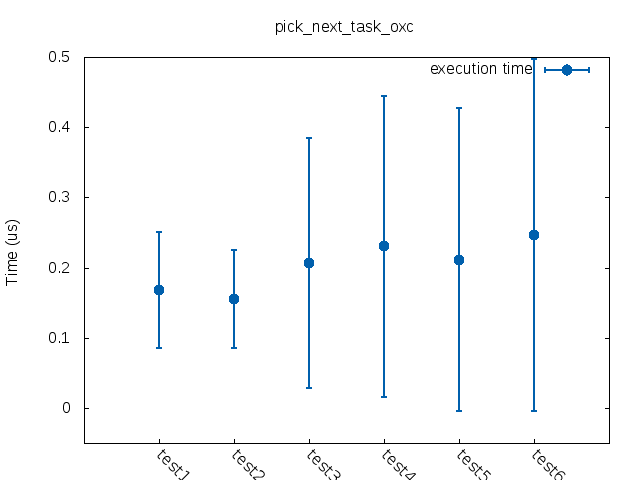
\includegraphics[width=\textwidth, totalheight=0.4\textheight]{images/pick_next_task_oxc}
        \caption{Measured execution time for \texttt{pick\_next\_task\_oxc}}
        \label{fig:pick_next}
\end{figure}
\begin{figure}[H]%htbp]
        \centering
        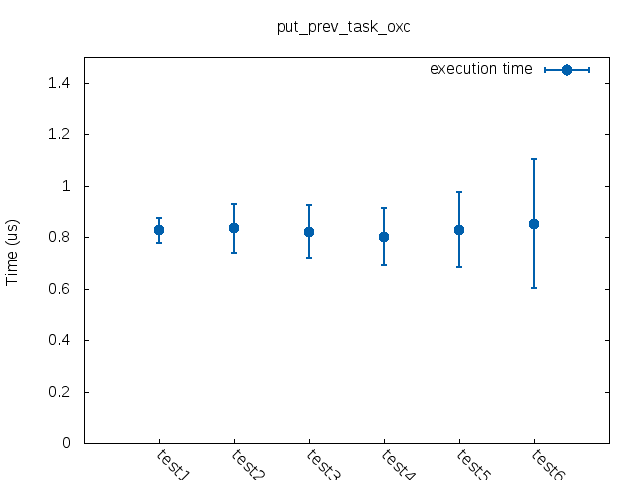
\includegraphics[width=\textwidth, totalheight=0.4\textheight]{images/put_prev_task_oxc}
        \caption{Measured execution time for \texttt{put\_prev\_task\_oxc}}
        \label{fig:put_prev}
\end{figure}
\begin{figure}[H]%htbp]
        \centering
        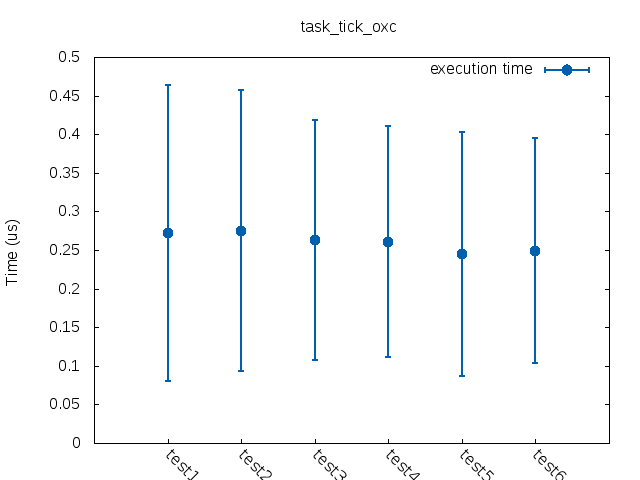
\includegraphics[width=\textwidth, totalheight=0.4\textheight]{images/task_tick_oxc}
        \caption{Measured execution time for \texttt{task\_tick\_oxc}}
        \label{fig:task_tick}
\end{figure}
Figure \ref{fig:pick_next} shows the statistical result of 
\texttt{pick\_next\_task\_oxc} in each test. One observation from the figure
is that with more ox containers joining the system, the time spent on executing
the function codes fluctuates more. This trend also reflects in the
results for \texttt{put\_prev\_task\_oxc}, as in figure \ref{fig:put_prev}.
However, figure \ref{fig:task_tick} for \texttt{task\_tick\_oxc} does not 
show this pattern.

Now we are going to probe why the execution time of \texttt{task\_tick\_oxc}
is more stable than the result of the other two. A look at the body of the
three functions in list \ref{list:pick_next}, \ref{list:put_prev} and
\ref{list:task_tick}, we can find that except for the enclosed scheduling
operations, other codes in the three functions are actually the same:
to update the per CPU runqueue, to update the per container runqueue and
update the current ox container. So, the different variance behaviour in 
measured execution time for oxc functions may be affected by the performance
of sheduling operations inside oxc container. 

The three encapsulated scheduling operations \texttt{pick\_next\_task\_rt}, 
\\\texttt{put\_prev\_task\_rt} and \texttt{task\_tick\_rt} are defined in
rt scheduling class. Specifically, the codes of \texttt{task\_tick\_rt},
which is called inside oxc function \texttt{task\_tick\_oxc}, is listed 
below. This is a very simple function. If people read the other two
scheduling operations' codes in \emph{linux/sched/rt.c}, this function is 
still less complex in dealing with runqueues. When scheduling operations 
are called inside an ox container, there will be extra cost because
the raw handle of implementation details, and such an influence may 
be smaller when the scheduling operation itself is simple. This explains 
why the result in \ref{fig:task_tick} is stable in both mean value and 
standard variance.
\begin{lstlisting}[language=C,
			caption={\texttt{task\_tick\_rt}},
			label={task_tick_rt}]
static void task_tick_rt(struct rq *rq, struct task_struct *p, int queued)
{
        update_curr_rt(rq);

        watchdog(rq, p);

        /*
         * RR tasks need a special form of timeslice management.
         * FIFO tasks have no timeslices.
         */
        if (p->policy != SCHED_RR)
                return;
        /*
         * The left part has no effects in our tests.
         */
        ...

}
\end{lstlisting}



\section{Experiment B}
\subsection{Experiment design}
The aim of this experiment is to estimate the overall overhead in oxc 
framework through comparison with non real-time CPU bandwidth control 
mechanisms that are already in Linux kernel. During tests the synthetic 
load is generated by the tbench benchmark tool. The CPU bandwidth 
allocated to tbench connections are allocated by oxc control, rt 
throttling and cfs bandwidth control individually. The tbench throughput 
results of oxc framework are then compared with rt throttling and cfs 
bandwidth control. By such comparisons, the overhead introduced by oxc 
control is then evaluated in a relative way.

Two tbench connections will be set up in the system.
Each connection will be dedicated to one CPU.
Without constraints, they will consume all CPU time.
In the experiment, the CPU bandwidth allocated to tbench traffic is restricted.
The per CPU bandwidth parameter used in tests includes
$0.05ms/1ms$, $0.1ms/1ms$, $0.2ms/1ms$, $0.4ms/1ms$, $0.6ms/1ms$ and 
$0.8ms/1ms$. 
Note that these are the per CPU bandwidth that is planned to assign to 
tbench tasks. Each cpu bandwidth control mechnism will restricts the 
tbench execution not exceed the configured value. And the throughput 
results will be proportional to the overhead in each bandwidth 
control mechanism.

When rt throttling is tested, tbench clients and servers will be 
scheduled as rt tasks with policy \texttt{SCHED\_RR}. Otherwise the client 
and server in the same connection cannot run at all. Correspondingly, to 
compare with rt throttling, tbench threads inside the ox container will 
be set as rt tasks with \texttt{SCHED\_RR} policy too. 
When comparing the oxc control with cfs bandwidth control, the tbench
threads inside ox containers will run as normal tasks. 

\subsection{Experiment results}
The thrughput results are shown in table \ref{tab:expB1} and \ref{tab:expB2}.
\begin{table}[H]%thbp]
	\centering
	\begin{tabular}{|l||c|c|}\hline
		 per CPU bandwidth & rt throttling & oxc control + rt scheduling\\\hline
			0.05/1ms &	21.9335	&	18.5313	\\\hline 
			0.1ms/1ms &	43.5794 &	36.89324 \\\hline
			0.2ms/1ms &	92.7356 &	73.5099	\\\hline
			0.4ms/1ms &	172.582 &	147.806 \\\hline
			0.6ms/1ms &	233	&	225.72	\\\hline
			0.8ms/1ms &	319.297 &	297.0607	\\\hline
	\end{tabular}
	\caption{Throughputs, in Mbps/sec, under rt throttling and oxc control}
	\label{tab:expB1}
\end{table}
\begin{table}[H]%thbp]
	\centering
	\begin{tabular}{|l||c|c|}\hline
		 per CPU bandwidth & cfs bandwidth control & oxc control + cfs scheduling  \\\hline
		 0.05ms/1ms	& 24.8825	& 19.2151 \\\hline
		 0.1ms/1ms	& 52.2106	& 39.4268 \\\hline
		 0.2ms/1ms	& 106.226	& 77.4225 \\\hline
		 0.4ms/1ms	& 215.071	& 151.465 \\\hline
		 0.6ms/1ms	& 323.628	& 234.369 \\\hline
		 0.8ms/1ms	& 433.025	& 305.1 \\\hline
	\end{tabular}
	\caption{Throughputs, in Mbps/sec, under cfs bandwidth and oxc control}
	\label{tab:expB2}
\end{table}
After a glance on the two tables, it's apparent to note that the 
throughput results under cfs bandwidth control outperform the other two. 
There are two reasons for this. Firstly, the overhead brought by cfs 
bandwidth control is indeed lower than the other two mechnanisms.
Secondly, both oxc tasks and rt tasks are more greedy than cfs tasks when 
they occupy a CPU. For oxc tasks, both rt and normal tasks are lower
priority tasks, between which normal tasks are lower priority tasks.
the oxc task or rt tasks will not give up a CPU to a lower priority
task until the CPU reservation is totally consumed. So lower priority 
tasks in the system are stressed more under oxc control or rt throttling, 
especially when high reservation parameter is configured. However, in cfs 
scheduling, cfs tasks, with or without CPU reservation, can share the CPU 
evenly.

\begin{figure}[htbp]
        \centering
        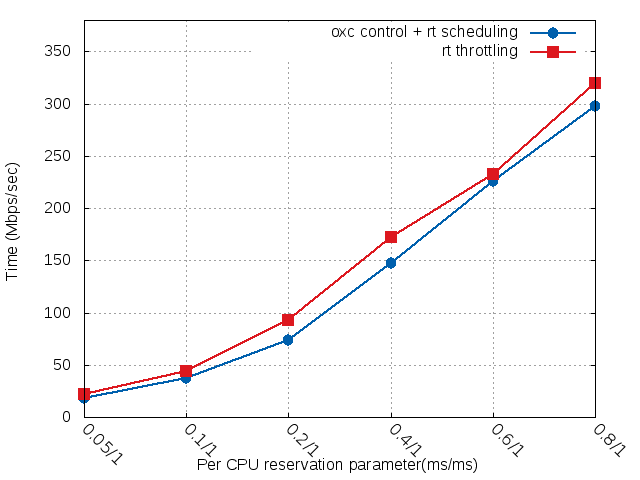
\includegraphics[width=\textwidth,totalheight=0.4\textheight]{images/expB1}
        \caption{\emph{oxc control} vs. \emph{rt throttling}}
        \label{fig:expB1}
\end{figure}
Having solved the above question, let's first study the peformance of tbench 
tasks in oxc framework when they are scheduled with \texttt{SCHED\_RR} 
policy. The comparison between oxc control and rt throttling in 
table \ref{tab:expB1} is visulized in figure \ref{fig:expB1}.
At first, the throughput result under rt throttling is higher and 
growing faster than the result in oxc control. However, as the more CPU 
bandwdith is reserved to tbench tasks, the throughtput results under the 
two means are converging. In fact, the throughtput growing trend in oxc 
control are consistent. When it comes to rt throttling, it's not like this.
When a relatively small fraction of CPU is assigned to rt throttling
and oxc control, rt throttling shows better performance. However, with
increasing the reserved CPU bandwdith, the stress of rt throttling on
the whole system is rising too, which slows growth of the throughput. 
Under oxc control, the throughput result is almost linear with the 
given reserved bandwidth. The overhead in oxc control behaves as 
a constant factor.

The comparason between oxc control and CPU bandwidth control is ahown 
in figure \ref{fig:expB2}. As we just analyzed, cfs bandwidth control has
much better throughput result. One observation is that althouth with
less rasing speed, the throughput increasing trend in oxc control has the
similar shape as in cfs bandwidth control. 
The result under oxc framework has another meaningful implication. 
When oxc control is used, allocations of bandwidth in the system should be
cautioned so as to achieve an optimal system performance. 

\begin{figure}[htbp]
        \centering
        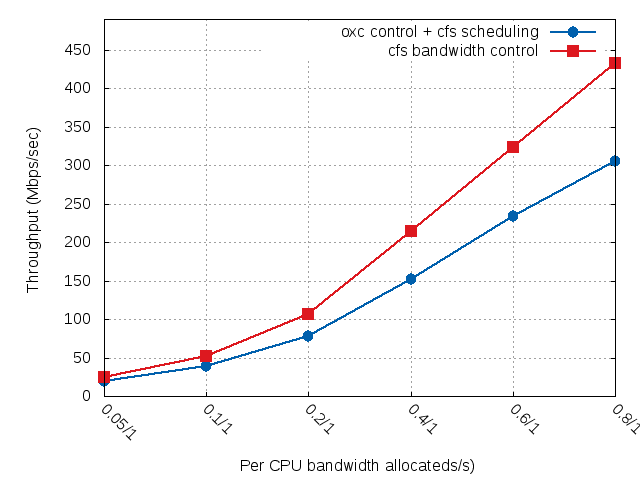
\includegraphics[width=\textwidth, totalheight=0.4\textheight]{images/expB2}
        \caption{\emph{oxc control} vs. \emph{cfs bandwidth control}}
        \label{fig:expB2}
\end{figure}
\begin{figure}[htbp]
        \centering
        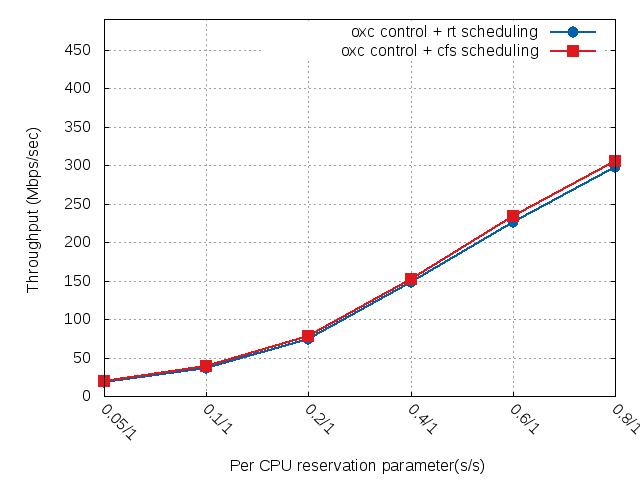
\includegraphics[width=\textwidth, totalheight=0.4\textheight]{images/expB3}
        \caption{\emph{oxc control + rt throttling} vs. \emph{oxc control + cfs scheduling}}
        \label{fig:expB3}
\end{figure}
At last, figure \ref{fig:expB3} mixes the statistics in table \ref{tab:expB1}
and \ref{tab:expB2} and draws the throughput results under oxc control with
rt throttling and cfs scheduling in the same graph.
The results are quite close, and the difference can be regarded as
the scheduling cost between rt and cfs scheduling in an ox container.
Still, cfs scheduling shows better results than rt scheduling even under 
oxc framework. This says that cfs scheduling introduces less overhead in the
system than rt scheduler. Such a comparison causes us to think about one
possible application of oxc framework. In some cases, when to compare two
schedulers, we can set up the environment inside an ox container; or by preparing
a certain number of ox containers, a lightweight networked testbed. 

\section{Experiment feedbacks}
The experiment does not show that the performance of oxc control is better than
existing bandwidth control methods. This is also not the experiment objective( the
comparison result with rt throttling is a small surprise). The experiment outcome
has an unstated meaning for future development of oxc framework.
Experiment A gives precise measurement of oxc function execution time and 
confirms the necessary to improve implementation quality of the oxc framework.
In experiment B, the overall performance of oxc framework is compared with
rt throttling and cfs bandwidth control. Its experiment analysis show us that
how to distribute CPU bandwidth will affect both the work inside an ox container
and the whole system behaviour; it also raises one example for oxc control usage. 
These feedbacks would be incorporated in the evolvement of the oxc framework.
